\documentclass[tikz,border=6pt]{standalone}
% tikz-style.tex (общий стиль для всех TikZ-картинок)
\RequirePackage[T1,T2A]{fontenc}
\RequirePackage[utf8]{inputenc}

% Palatino-подобный шрифт (как в MathJax часто воспринимается «более вытянутым»)
\RequirePackage{txfonts}
% txfonts даёт предупреждение по кириллице (T2A/txr не определён).
% Оставляем txfonts для математики, а текстовый шрифт возвращаем на Computer Modern,
% чтобы не искать T2A/txr и убрать предупреждения.
\renewcommand{\rmdefault}{cmr}
\renewcommand{\sfdefault}{cmss}
\renewcommand{\ttdefault}{cmtt}

\RequirePackage{tikz}
\RequirePackage{xcolor}
\usetikzlibrary{calc}

% цвета
\definecolor{lightgreen}{RGB}{214,234,214}
\definecolor{darkgreen}{HTML}{0B7A0B}
\definecolor{darkred}{HTML}{DF0000}

\definecolor{midgreen}{HTML}{2E9B2E}
\definecolor{palegreen}{RGB}{235,246,235}
\definecolor{olivegreen}{HTML}{3E6B2F}

\definecolor{lightred}{RGB}{255,220,220}
\definecolor{midred}{HTML}{E04545}
\definecolor{darkred2}{HTML}{A80000}

\definecolor{lightblue}{RGB}{220,232,255}
\definecolor{midblue}{HTML}{2E5BD6}
\definecolor{darkblue}{HTML}{0B2E8A}

\definecolor{lightgray}{RGB}{240,240,240}
\definecolor{midgray}{RGB}{170,170,170}
\definecolor{darkgray}{RGB}{80,80,80}

\definecolor{vtxfill}{RGB}{86,193,255}
\definecolor{vennfill}{RGB}{220,232,255}


% единый набор стилей TikZ
\tikzset{
    lab/.style={
        font=\fontsize{24}{32}\selectfont
    }
}


\begin{document}
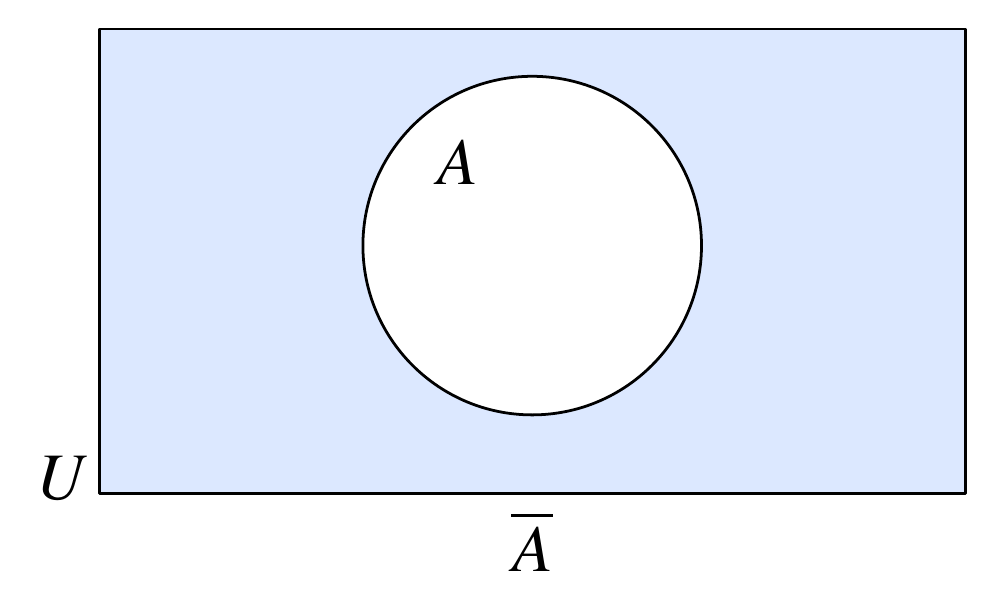
\begin{tikzpicture}[line cap=round,line join=round]

% --- geometry (tuned to match the reference) ---
    \def\R{2.15}                 % circle radius
    \coordinate (C) at (0,0.20); % circle center

% shaded universe rectangle (filled)
    \fill[vennfill] (-5.5,-2.95) rectangle (5.5,2.95);
    \draw[line width=1.0pt] (-5.5,-2.95) rectangle (5.5,2.95);

% set A (white circle on top of the fill)
    \fill[white] (C) circle (\R);
    \draw[line width=1.0pt] (C) circle (\R);

% label A inside the circle (top-left)
    \node[lab] at ($ (C) + (-0.95,1.05) $) {$A$};

% caption below (centered under the rectangle)
    \node[lab] at (0,-3.55) {$\overline{A}$};
% universe label U (outside bottom-left of the rectangle)
    \node[lab, anchor=north east] at (-5.5,-2.35) {$U$};

  \end{tikzpicture}
\end{document}